\section[WP4: Implementazione e valutazione sperimentale]{WP\,4: Implementazione e valutazione sperimentale}
\label{wp4:implementazione-valutazione}

Il quarto work package realizza un prototipo locale del protocollo definito nei WP precedenti e ne valuta il comportamento mediante test e benchmark. L'obiettivo non \`e produrre un sistema pronto per l'impiego operativo, ma verificare che le scelte progettuali siano implementabili in modo coerente e osservabile: configurazione dell'elezione, autorizzazione pseudonima, deposito e sostituzione del voto, chiusura, scrutinio, verifica individuale, verifica pubblica e misure prestazionali.

\subsection{Obiettivi e perimetro del prototipo}
\label{wp4:obiettivi-perimetro}

Il prototipo \`e locale, stand-alone e privo di servizi di rete o database esterni. Gli attori del protocollo sono separati logicamente mediante moduli, chiavi e responsabilit\`a distinte, ma l'esecuzione avviene nello stesso ambiente applicativo e le interazioni sono realizzate tramite chiamate locali.

Il perimetro comprende il flusso completo necessario alla dimostrazione: setup dell'elezione, emissione dell'autorizzazione, preparazione del pacchetto di voto, validazione del Bulletin Board, sostituzione entro $V_{\max}$, chiusura, scrutinio e verifiche. Restano fuori dal prototipo l'infrastruttura distribuita reale, canali TLS operativi, isolamento fisico tra server, database remoti, gestione production delle credenziali, mitigazioni complete contro indisponibilit\`a e attacchi di rete.

\subsection{Architettura dell'implementazione}
\label{wp4:architettura}

\subsubsection{Attori logici}

L'implementazione modella gli stessi ruoli del protocollo: Registration Authority, Bulletin Board, Tallying Authority, elettore, commissari elettorali e verificatore pubblico. La Registration Authority autentica gli aventi diritto fittizi e rilascia una sola autorizzazione pseudonima per elezione. Il Bulletin Board valida pacchetti, mantiene il registro append-only, emette ricevute e registra la chiusura. La Tallying Authority custodisce la chiave di scrutinio protetta, seleziona le schede finali e firma il risultato. I commissari custodiscono le quote Shamir necessarie a ricostruire $K_{\mathit{wrap}}$.

\subsubsection{Moduli principali}

Il codice \`e organizzato in moduli con responsabilit\`a separate. I modelli definiscono le strutture dati pubbliche e interne; la serializzazione canonica produce rappresentazioni deterministiche per hash e firme; le primitive crittografiche raccolgono cifratura, firme, hash, password, protezione dello stato locale, $\mathit{blob}_{\mathit{TA}}$ e Shamir. I moduli degli attori implementano RA, BB, TA, elettore e commissari; la persistenza gestisce archivi locali e stato cifrato dell'elettore; il workflow coordina la dimostrazione end-to-end; la GUI offre una vista dimostrativa locale; i benchmark misurano operazioni crittografiche e applicative senza modificare il protocollo.

Tutti i dati firmati o sottoposti a digest usano una serializzazione canonica comune, cos\`i da evitare ambiguit\`a tra produttore e verificatore. La separazione dei moduli consente inoltre di testare singolarmente primitive, regole del Bulletin Board, persistenza, scrutinio e verifiche pubbliche.

\subsection{Configurazione e setup dell'elezione}
\label{wp4:configurazione-setup}

Il setup genera chiavi distinte per i ruoli che devono firmare o decifrare: RA, BB, TA per la cifratura e TA per la firma. La coppia $(\pk_{\mathit{TA\_enc}}, \sk_{\mathit{TA\_dec}})$ \`e usata per la cifratura e decifratura dei voti; la coppia $(\pk_{\mathit{TA\_sig}}, \sk_{\mathit{TA\_sig}})$ firma i parametri pubblici e il risultato finale.

I parametri pubblici dell'elezione sono serializzati in forma canonica e includono il contesto, la versione, $\mathit{election\_id}$, le liste ammesse, apertura e chiusura, numero di aventi diritto, $V_{\max}$, soglia $(t,n)$ e chiavi pubbliche TA, RA e BB. Da tale payload si calcola $\mathit{params\_hash}$ e la TA produce $\mathit{SIG}_{\mathit{params}}$ con $\sk_{\mathit{TA\_sig}}$. I componenti del prototipo ricalcolano l'hash e verificano la firma con $\pk_{\mathit{TA\_sig}}$ prima di procedere.

Nel profilo dimostrativo il limite di sostituzione \`e $V_{\max}=3$ e la custodia distribuita usa Shamir con soglia $t=3$ su $n=5$ quote. La chiave privata $\sk_{\mathit{TA\_dec}}$ non viene divisa direttamente: viene protetta in $\mathit{blob}_{\mathit{TA}}$ mediante $K_{\mathit{enc}}$ e $K_{\mathit{mac}}$, derivate da $K_{\mathit{wrap}}$. Il segreto $K_{\mathit{wrap}}$ \`e poi distribuito ai commissari tramite Shamir.

\subsection{Registrazione e persistenza dello stato elettore}
\label{wp4:registrazione-persistenza}

La RA mantiene un archivio locale riservato di elettori fittizi aventi diritto. Le password non sono conservate in chiaro: per ciascun elettore viene registrato un verificatore derivato con salt casuale e parametri persistiti.

L'elettore genera localmente il segreto $t_i$, lo pseudonimo $p_i = H(t_i)$ e la coppia pseudonima $(\pk_i^{\mathit{vote}}, \sk_i^{\mathit{vote}})$. La richiesta di autorizzazione contiene $\mathit{election\_id}$, $p_i$ e $\pk_i^{\mathit{vote}}$; la RA la firma con RSA-PSS e rilascia $\tau_i$ una sola volta per elettore ed elezione.

Lo stato locale dell'elettore contiene le informazioni necessarie a votare e sostituire il voto: segreto $t_i$, pseudonimo, chiave pseudonima, autorizzazione, versione corrente e ricevute. Tale stato \`e cifrato con AES-256-GCM e pu\`o essere recuperato dopo la riapertura dell'applicazione. Se lo stato viene perso o corrotto, l'elettore non pu\`o costruire una sostituzione valida; inoltre la RA non rilascia una seconda autorizzazione per la stessa elezione. La scheda gi\`a accettata dal Bulletin Board resta quindi valida e scrutinabile.

\subsection{Deposito e sostituzione del voto}
\label{wp4:deposito-sostituzione}

Il voto viene preparato cifrando il codice della lista scelta con RSA-OAEP e la chiave pubblica $\pk_{\mathit{TA\_enc}}$. Il pacchetto include ciphertext, pseudonimo, chiave pubblica pseudonima, autorizzazione RA, versione e firma pseudonima RSA-PSS. La firma vincola il pacchetto alla coppia pseudonima dell'elettore e alla serializzazione canonica del messaggio.

Il Bulletin Board accetta un pacchetto solo se risultano validi l'identificativo di elezione, la finestra temporale, l'autorizzazione RA, la firma pseudonima, la chiave pubblica associata allo pseudonimo, la versione e il limite $V_{\max}=3$. I replay identici sono rilevati e non producono nuove entry.

Prima della chiusura, una sostituzione \`e ammessa soltanto con lo stesso $p_i$, la stessa autorizzazione, la stessa chiave pseudonima e una versione consecutiva non superiore a $V_{\max}$. Le versioni precedenti non vengono cancellate: rimangono nel registro append-only, ma per lo scrutinio viene selezionata solo la versione valida pi\`u alta registrata prima di $\texttt{CLOSE}$.

\subsection{Bulletin Board, chiusura e scrutinio}
\label{wp4:bb-chiusura-scrutinio}

Ogni voto accettato diventa un record pubblico del Bulletin Board. Il relativo $\mathit{RID}_i$ \`e calcolato con SHA-256 sulla rappresentazione canonica dei campi rilevanti del pacchetto. Il registro \`e append-only: ciascun record contiene indice, hash precedente, hash dell'entry e valore corrente della hash chain. In caso di accettazione, il BB emette una ricevuta firmata che lega $\mathit{election\_id}$, indice, $\mathit{RID}_i$ e stato della catena.

Alla chiusura il Bulletin Board aggiunge un record $\texttt{CLOSE}$, calcola $h_{\mathit{close}}$ e firma lo stato finale del registro. Dopo tale evento non sono accettati nuovi voti o sostituzioni.

Lo scrutinio opera solo sulle versioni finali valide. La TA apre $\mathit{blob}_{\mathit{TA}}$ solo dopo la ricostruzione di $K_{\mathit{wrap}}$ con almeno $t$ quote Shamir valide; l'apertura \`e autenticata e verifica il MAC prima della decifratura. Le schede finali sono decifrate con la chiave privata $\sk_{\mathit{TA\_dec}}$ recuperata temporaneamente. Plaintext malformati o fuori dominio sono classificati come anomalie. Il risultato contiene i totali per lista, il numero di schede finali, il numero di schede valide e le anomalie, ed \`e firmato dalla TA con $\sk_{\mathit{TA\_sig}}$.

\subsection{Verifica individuale e pubblica}
\label{wp4:verifica}

La verifica individuale consente all'elettore di controllare la propria ricevuta firmata dal BB e l'inclusione della scheda cifrata nel registro. Il controllo riguarda $\mathit{election\_id}$, indice, $\mathit{RID}_i$, hash di catena, firma della ricevuta e coerenza con il registro verificato.

La verifica pubblica controlla $\mathit{params\_hash}$ e $\mathit{SIG}_{\mathit{params}}$, firme RA sulle autorizzazioni, firme pseudonime sui pacchetti, $\mathit{RID}_i$ ricalcolati, indici e hash chain, versioni consecutive, limite $V_{\max}$, selezione delle ultime versioni valide, presenza e firma del record $\texttt{CLOSE}$, legame del risultato con $h_{\mathit{close}}$, firma TA del risultato e coerenza numerica:
\[
\sum_j N_j + N_{\mathit{anomale}} = N_{\mathit{entry\_finali}}.
\]

Questa verifica non decifra i voti e non fornisce una prova pubblica della corretta decifratura di ogni singolo ciphertext. La propriet\`a ottenuta \`e quindi una verificabilit\`a pubblica parziale, coerente con i limiti gi\`a dichiarati nel WP3.

\subsection{Workflow dimostrativo e interfaccia grafica}
\label{wp4:workflow-gui}

Il workflow dimostrativo esegue l'intero ciclo locale: configurazione del profilo demo, verifica della firma TA sui parametri pubblici, registrazione di elettori fittizi, emissione delle autorizzazioni, salvataggio e riapertura dello stato cifrato, deposito dei voti, sostituzione valida, chiusura del BB, scrutinio, verifica delle ricevute, verifica del registro e verifica del risultato.

L'interfaccia grafica \`e locale e dimostrativa. Usa quattro schede: configurazione, elettori e voto, Bulletin Board, scrutinio e verifica. La GUI non introduce servizi esterni; espone una vista controllata del workflow e mostra solo informazioni pubbliche o abbreviate, come prefissi di hash, pseudonimi e $\mathit{RID}_i$. Non visualizza chiavi private, segreti elettore, $K_{\mathit{wrap}}$, quote Shamir, ciphertext completi o collegamenti identit\`a--pseudonimo--voto.

Le quattro schermate principali della dimostrazione sono riportate nelle Figure~\ref{wp4:fig-gui-configurazione}, \ref{wp4:fig-gui-elettori-voto}, \ref{wp4:fig-gui-bulletin-board} e \ref{wp4:fig-gui-scrutinio-verifica}.

\begin{figure}[H]
\centering
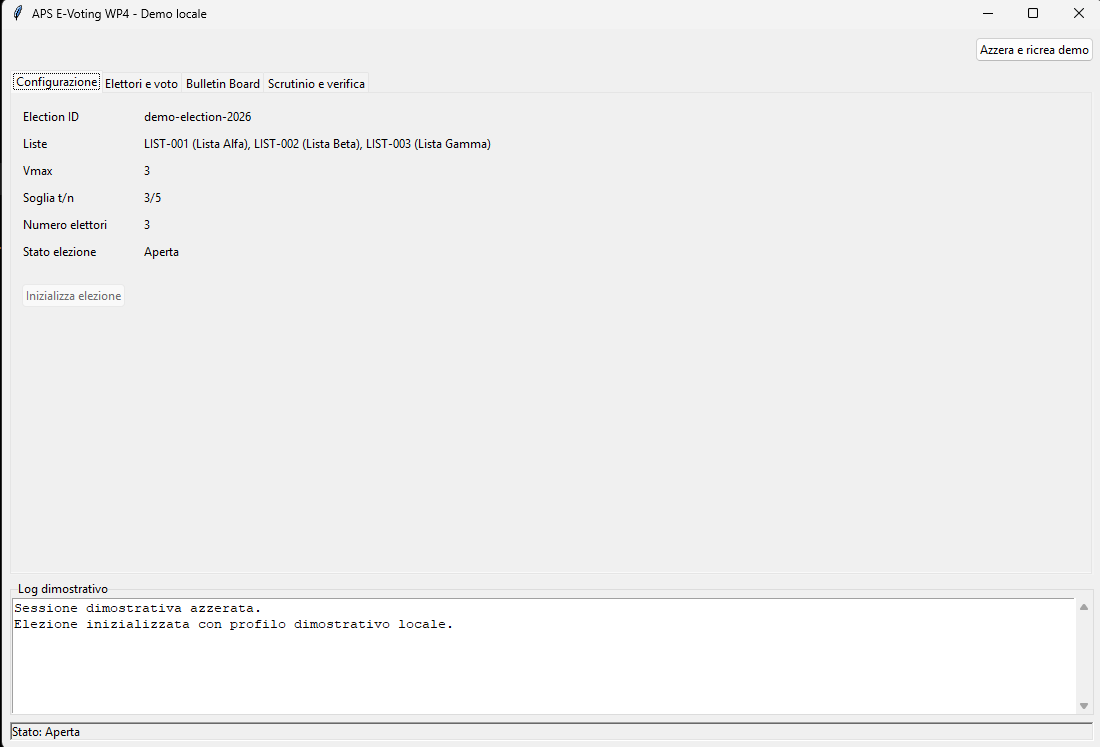
\includegraphics[width=0.92\textwidth]{Figures/gui-configurazione.png}
\caption{Configurazione iniziale del profilo dimostrativo: liste ammesse, limite Vmax, soglia Shamir ed elettori.}
\label{wp4:fig-gui-configurazione}
\end{figure}

\begin{figure}[H]
\centering
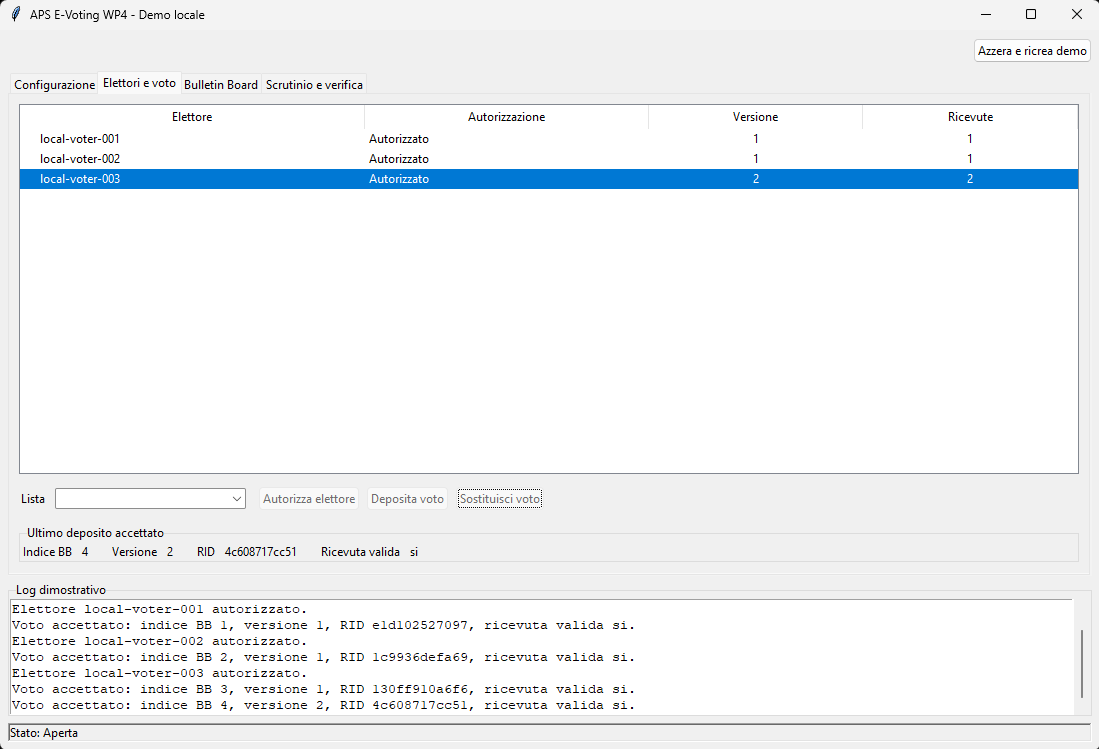
\includegraphics[width=0.92\textwidth]{Figures/gui-elettori-voto.png}
\caption{Stato degli elettori dopo tre depositi e una sostituzione del voto.}
\label{wp4:fig-gui-elettori-voto}
\end{figure}

\begin{figure}[H]
\centering
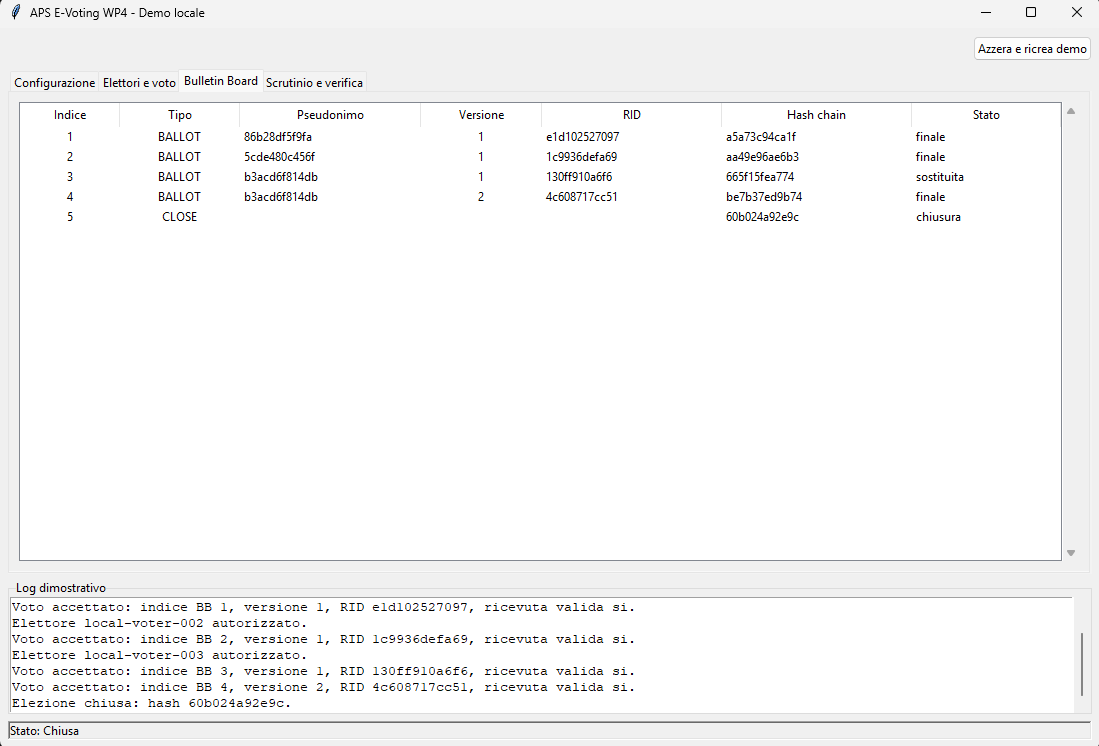
\includegraphics[width=0.92\textwidth]{Figures/gui-bulletin-board.png}
\caption{Bulletin Board dopo la sostituzione e la chiusura: record BALLOT, versione sostituita e record CLOSE.}
\label{wp4:fig-gui-bulletin-board}
\end{figure}

\begin{figure}[H]
\centering
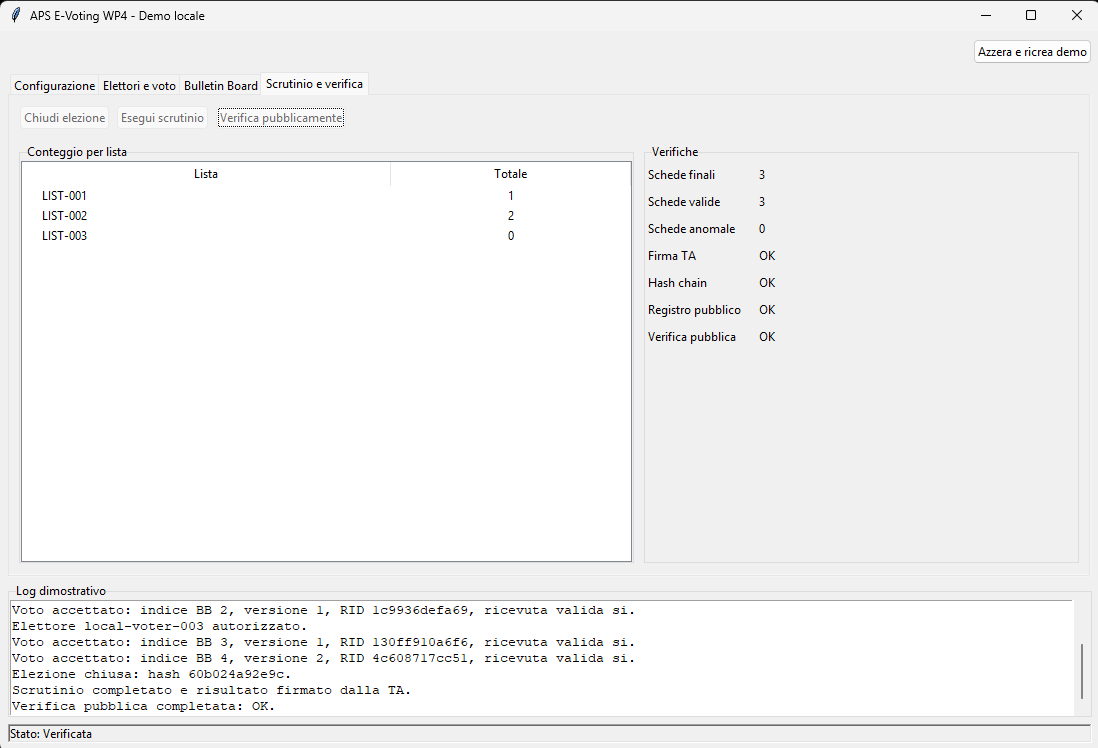
\includegraphics[width=0.92\textwidth]{Figures/gui-scrutinio-verifica.png}
\caption{Risultato dello scrutinio e completamento delle verifiche pubbliche.}
\label{wp4:fig-gui-scrutinio-verifica}
\end{figure}

\subsection{Strategia e risultati dei test}
\label{wp4:test}

La suite finale contiene 282 test superati. La copertura \`e organizzata in quattro gruppi principali.

\begin{itemize}
\item Test unitari: modelli, serializzazione canonica, hash, cifratura RSA-OAEP, firme RSA-PSS, password, Shamir, $\mathit{blob}_{\mathit{TA}}$, stato cifrato dell'elettore e formattazione dei dati pubblici.
\item Test di integrazione: workflow completo, registrazione, autorizzazione, voto, sostituzione, chiusura, scrutinio, verifica individuale, verifica pubblica e flusso GUI locale.
\item Test di sicurezza: alterazione dei parametri pubblici, firma TA errata o prodotta con chiave diversa, autorizzazioni contraffatte, firme modificate, replay, versioni non valide, superamento di $V_{\max}$, voto dopo $\texttt{CLOSE}$, hash chain manomessa, quote Shamir duplicate o malformate, $\mathit{blob}_{\mathit{TA}}$ alterato, MAC non valido, ciphertext malformati e plaintext fuori dominio.
\item Test benchmark: profilo rapido per verificare schema dei risultati, metriche non negative e assenza di dati riservati negli output di misura.
\end{itemize}

Sono inclusi test specifici sulla perdita o corruzione dello stato elettore. Tali casi verificano che la sostituzione non possa essere prodotta senza lo stato locale valido, che la RA rifiuti una seconda autorizzazione e che la scheda gi\`a accettata resti disponibile per lo scrutinio.

\subsection{Benchmark e valutazione delle prestazioni}
\label{wp4:benchmark}

I benchmark sono stati eseguiti con Python 3.14.5 su Windows 11 Home 64 bit, Intel Core i7-12700H e 16 GB di RAM. Il profilo completo usa una fase di warm-up e 5 ripetizioni per le operazioni temporali; i tempi sono riportati in millisecondi. I valori seguenti riprendono le mediane e le dimensioni indicate nel report sperimentale, senza ricalcoli.

\begin{table}[H]
\centering
\resizebox{\textwidth}{!}{%
\begin{tabular}{>{\raggedright\arraybackslash}p{5.1cm}
                >{\raggedright\arraybackslash}p{4.7cm}
                r
                r}
\toprule
\textbf{Operazione} & \textbf{Input / scala} & \textbf{Mediana ms} & \textbf{Dimensione byte} \\
\midrule
Generazione chiave RSA per firma & $2048$ bit & 37.8399 & 0 \\
Generazione chiave RSA per cifratura & $2048$ bit & 46.8595 & 0 \\
Autenticazione e autorizzazione RA & $scrypt\_n=32768$ & 93.3756 & 256 \\
Cifratura RSA-OAEP del voto & plaintext di 8 byte & 0.0263 & 256 \\
Firma RSA-PSS del pacchetto & messaggio di 1114 byte & 0.4765 & 256 \\
Preparazione completa del pacchetto & singolo pacchetto voto & 30.6746 & 1814 \\
Validazione e accettazione BB & singolo pacchetto voto & 1.0974 & 1814 \\
Aggiornamento hash chain & singolo collegamento & 0.0287 & 1966 \\
Verifica ricevuta BB & singola ricevuta & 0.0441 & 568 \\
Suddivisione Shamir & soglia $3$, quote $5$, segreto 32 byte & 0.0083 & 0 \\
Ricostruzione Shamir & soglia $3$, quote fornite $3$ & 0.0073 & 0 \\
Creazione $\mathit{blob}_{\mathit{TA}}$ & chiave privata serializzata di 1704 byte & 0.0786 & 162 \\
Apertura $\mathit{blob}_{\mathit{TA}}$ & soglia $3$, quote fornite $3$ & 0.0607 & 162 \\
Scrutinio & 10 schede finali & 35.2956 & 614 \\
Dimensione pacchetto voto & singolo pacchetto voto & 0.0000 & 1814 \\
Dimensione ricevuta & singola ricevuta & 0.0000 & 568 \\
\bottomrule
\end{tabular}%
}
\caption{Benchmark WP4: sintesi delle operazioni principali.}
\label{wp4:tab-benchmark-operazioni}
\end{table}

Le righe relative alla dimensione del pacchetto e della ricevuta non rappresentano operazioni temporali; per questo motivo il tempo \`e riportato come $0.0000$ ms. Anche la generazione delle chiavi RSA \`e misurata separatamente e non viene sommata alle operazioni ordinarie di voto.

\begin{table}[H]
\centering
\begin{tabular}{r r r r r r}
\toprule
\textbf{Eventi} & \textbf{Rip.} & \textbf{Min ms} & \textbf{Mediana ms} & \textbf{Media ms} & \textbf{Dev. std ms} \\
\midrule
2  & 5 & 0.2966 & 0.3082 & 0.3271 & 0.0531 \\
4  & 5 & 0.5810 & 0.6007 & 0.5985 & 0.0159 \\
11 & 5 & 1.5735 & 1.6055 & 1.7260 & 0.1914 \\
26 & 5 & 3.9386 & 3.9958 & 4.1199 & 0.2329 \\
\bottomrule
\end{tabular}
\caption{Benchmark WP4: verifica pubblica su registri di dimensione crescente.}
\label{wp4:tab-benchmark-verifica-pubblica}
\end{table}

La verifica pubblica cresce in modo coerente con il numero di eventi esaminati, poich\'e il verificatore ricalcola record, firme, $\mathit{RID}_i$, hash chain, versioni, selezione finale e coerenza numerica. I risultati devono tuttavia essere letti come misure del prototipo locale e non come stima di un sistema distribuito reale.

\subsection{Limiti del prototipo}
\label{wp4:limiti}

Il prototipo conserva limiti espliciti. La verifica pubblica della corretta decifratura resta parziale: registro, firme, versioni, $V_{\max}$, selezione finale, legame con $h_{\mathit{close}}$, firma TA e coerenza numerica sono controllabili, ma non sono presenti prove pubbliche della corretta decifratura di ogni scheda.

Non \`e implementata una vera threshold decryption. Shamir protegge $K_{\mathit{wrap}}$, ma durante lo scrutinio la chiave privata di decifratura della TA viene ricostruita temporaneamente nell'ambiente della TA. La GUI ha finalit\`a dimostrativa e non sostituisce un'interfaccia di produzione. La persistenza \`e limitata allo scenario locale e non include un database distribuito o politiche operative complete. I benchmark, infine, sono stati raccolti su una singola macchina e non rappresentano latenza di rete, concorrenza reale, isolamento tra server o carichi di un'infrastruttura distribuita.

\subsection{Considerazioni conclusive}
\label{wp4:conclusioni}

Il WP4 mostra che il protocollo descritto nei WP precedenti pu\`o essere implementato in un prototipo locale coerente con le propriet\`a progettuali principali. La separazione logica degli attori, l'uso di serializzazione canonica, firme, cifratura probabilistica, registro append-only, Shamir su $K_{\mathit{wrap}}$, persistenza cifrata dello stato elettore e verifiche pubbliche consentono di esercitare l'intero workflow in modo riproducibile.

La suite di test conferma il comportamento atteso nei casi ordinari e in numerosi casi negativi. I benchmark indicano costi contenuti per le operazioni locali misurate, con particolare attenzione alla separazione tra primitive crittografiche, operazioni applicative e verifica pubblica. Le limitazioni dichiarate rimangono sostanziali e impediscono di interpretare il prototipo come sistema elettorale reale; esso costituisce invece una validazione didattica e sperimentale del disegno protocollare.
